\subsection{Voxelization}\paragraph{}
Normally a volume is populated using some provided static 3D texture data.  For our implementation we manually update individual voxel ourselves. 

The goal of our voxelization method is to properly populate our volume. We want the shape of our final voxels represent the billowing, semi-spherical shape of a cloud. Not only do we desire the proper shape, we also aim to highlight the voxels nearest to the light source. 

We do our voxelization using billboards and a multi-pass voxelization system. One every frame we clear the entire volume and rerun a full voxelization pass. This will be essential if we ever add procedurally animated clouds. 

\subsubsection{Spherical Billboards}\paragraph{}
We begin by rendering many billboards from the light's perspective. In the billboard's fragment shader we calculate a spherical distribution mapped to the face of the billboard. Using this spherical distribution, we populate a sphere in the volume. 

% Code defining inital spherical voxelization
\begin{lstlisting}[caption={first\_voxelize.glsl, 42}]
// Calculate distance from the current fragment to billboard's center
float dist = distance(center, fragPos);
// Calculate linear distribution [0, 1]
float distribution = distToCenter / radius;
// Convert linear distribution to spherical [0, 1]
distribution = sqrt(max(0, 1 - distribution * distribution));
// Calculate the near point of the sphere intersecting this fragment
float sphereDistance = radius * distribution;
vec3 nearPos = fragPos + billboardNormal * sphereDistance;
// Iterate from front to back, voxelize along the way
for(float length = 0; length < 2 * sphereDistance; length += stepSize) {
	vec3 worldPos = nearPos - billboardNormal * length;
	imageStore(volume, getVoxelIndex(worldPos), vec4(0,0,0,1));
}
\end{lstlisting}\paragraph{}

% Voxelization figures
\begin{figure}[t]
\centering
	% Spherical distribution mapped to a billboard
	\begin{subfigure}[t]{0.48\textwidth}
	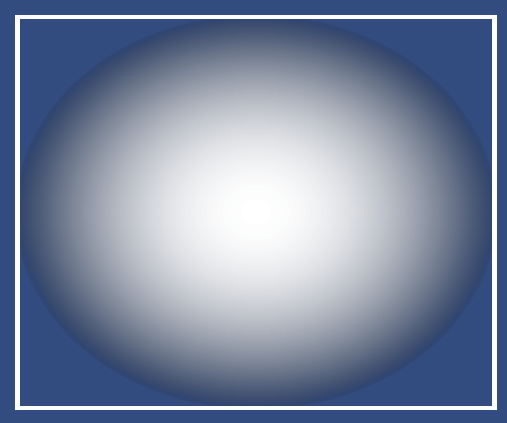
\includegraphics[width=\textwidth]{../res/spherebillboard.png}
	\caption{Spherical distribution mapped to a billboard}
	\end{subfigure}
	~
	% light-facing spherical billboard(s)
	\begin{subfigure}[t]{0.48\textwidth}
	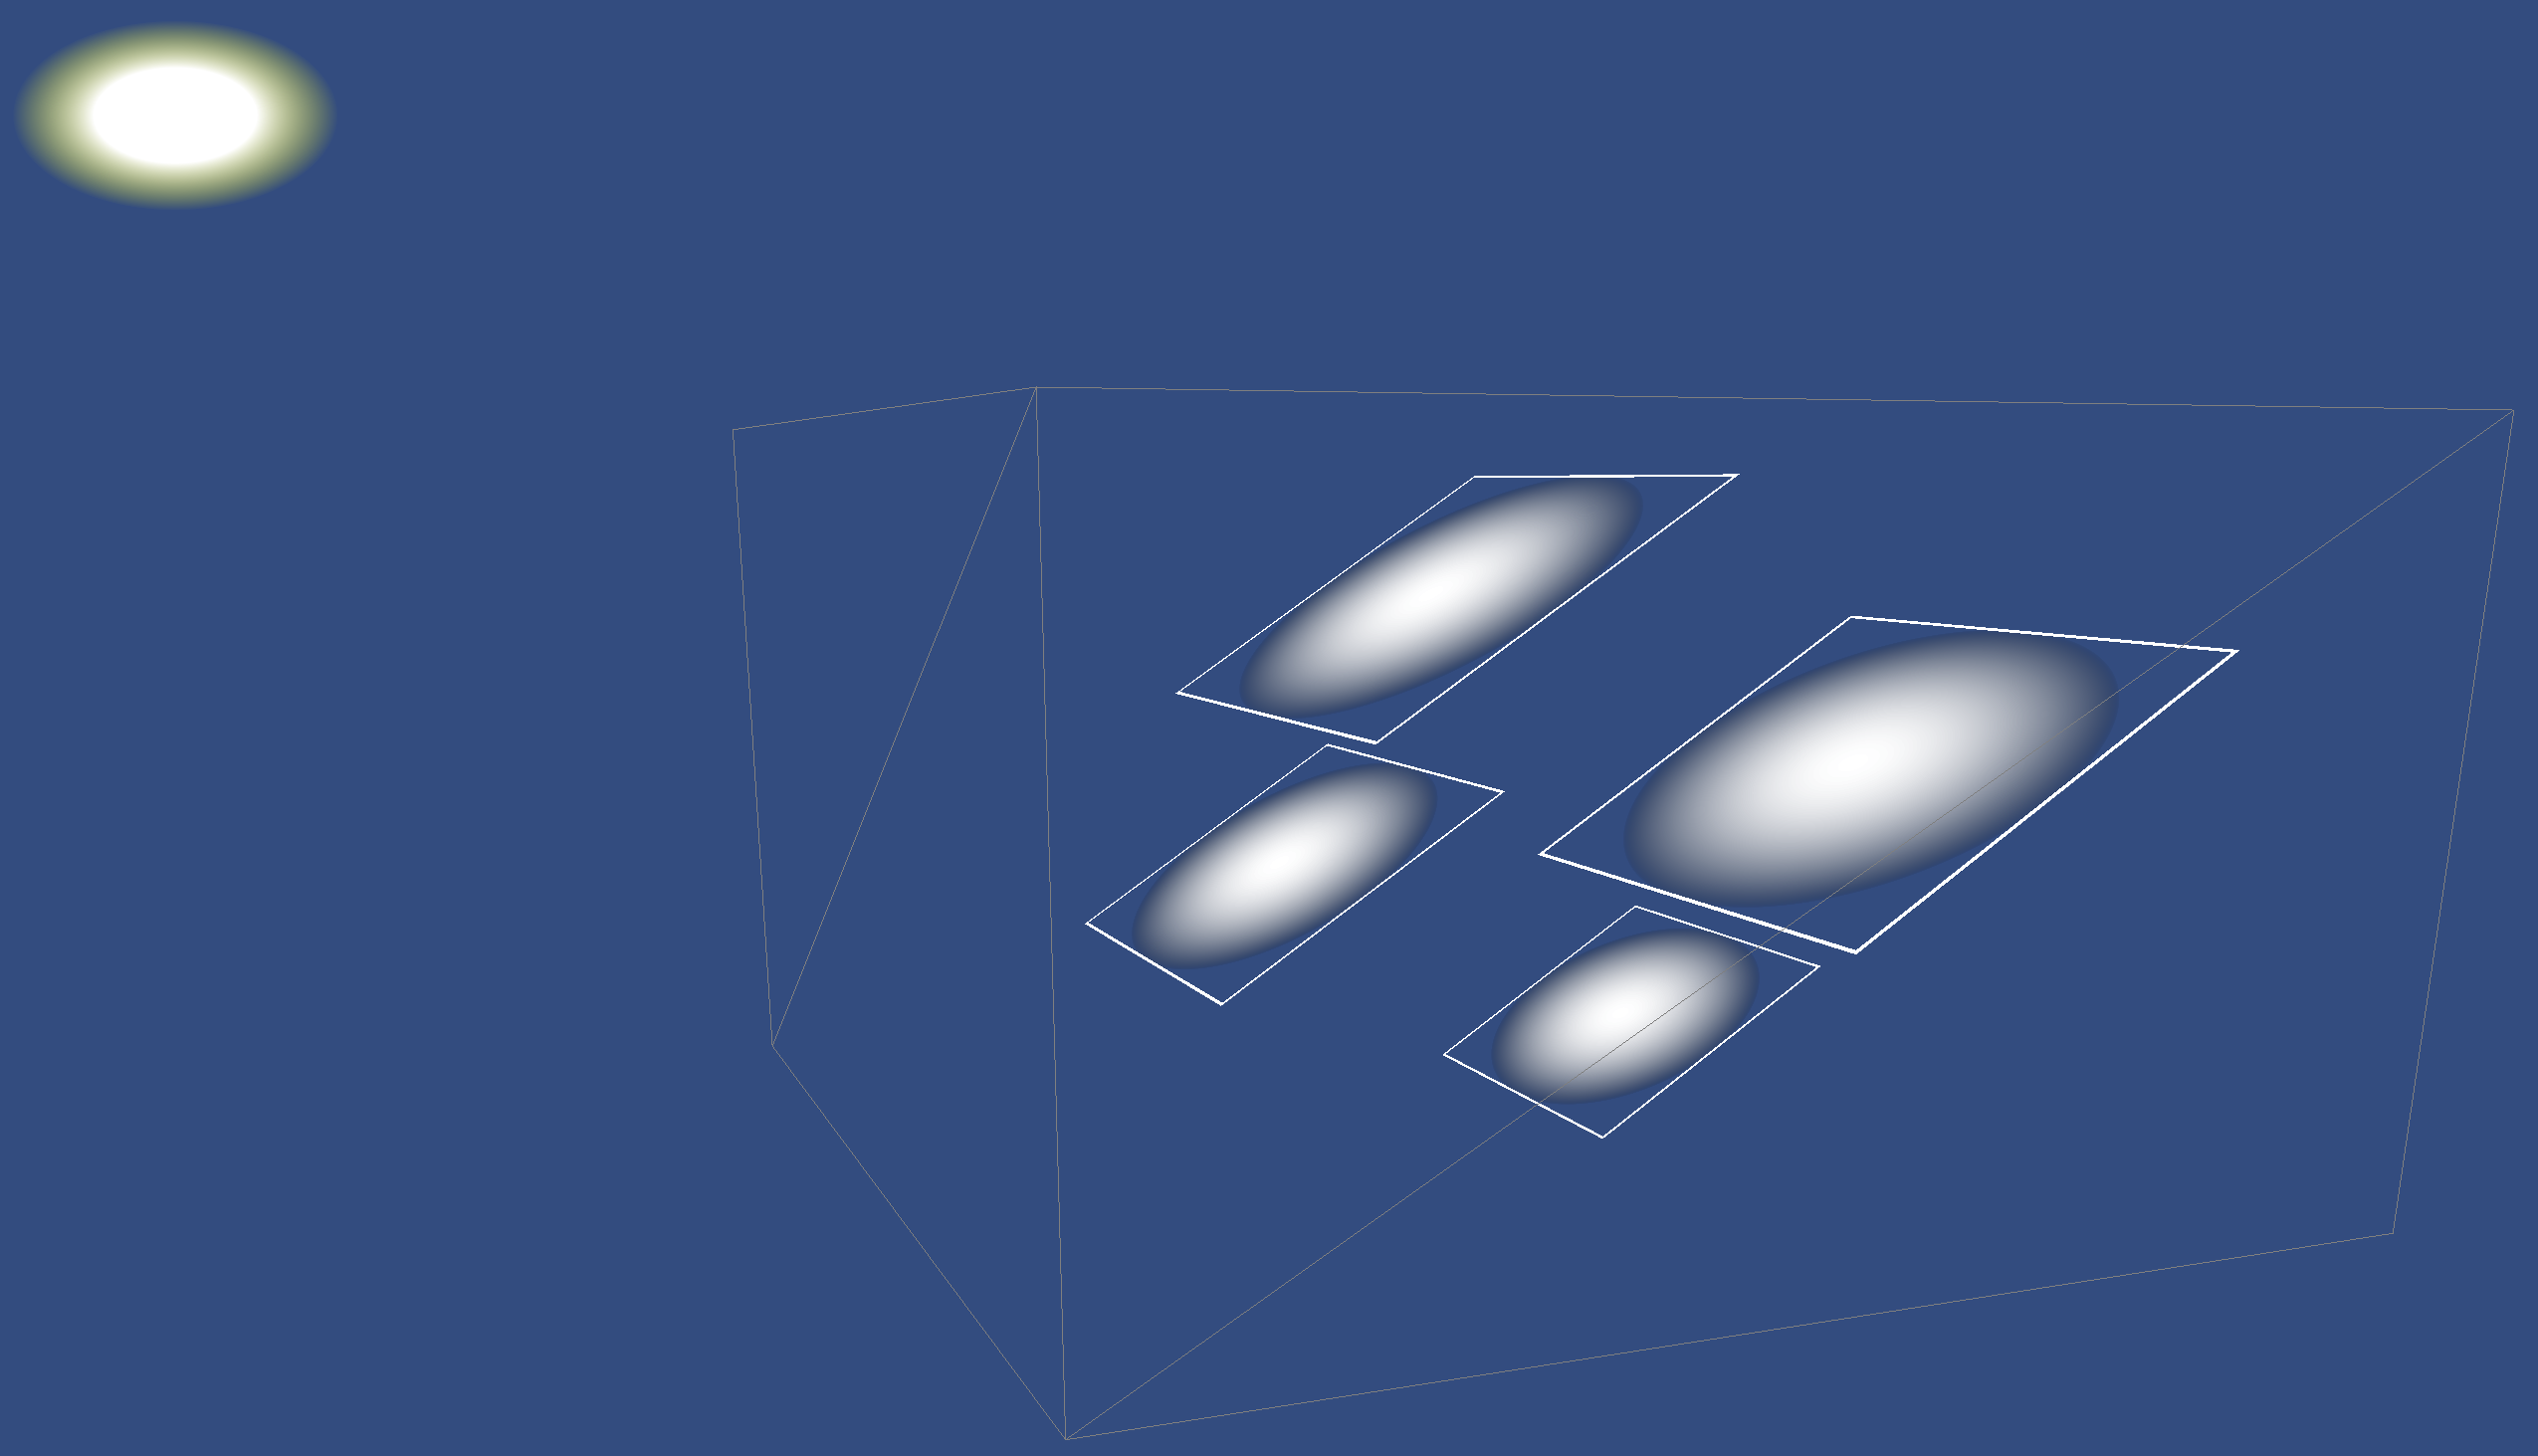
\includegraphics[width=\textwidth]{../res/lightfacing.png}
	\caption{Light-facing billboards}
	\end{subfigure}
	~
	% TODO : diagram
	\begin{subfigure}[t]{0.48\textwidth}
	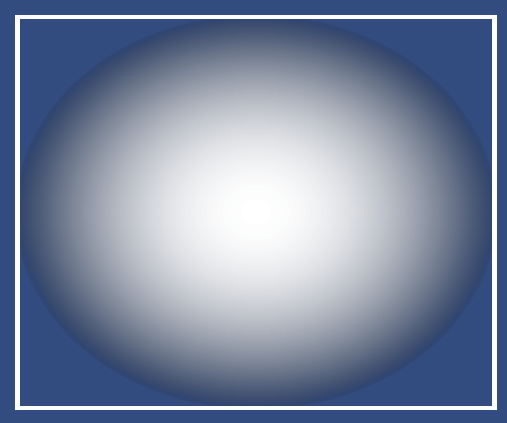
\includegraphics[width=\textwidth]{../res/spherebillboard.png}
	\caption{Diagram of spherical voxelization}
	\end{subfigure}
	~
	% Voxelization of light-facing billboards
	\begin{subfigure}[t]{0.48\textwidth}
	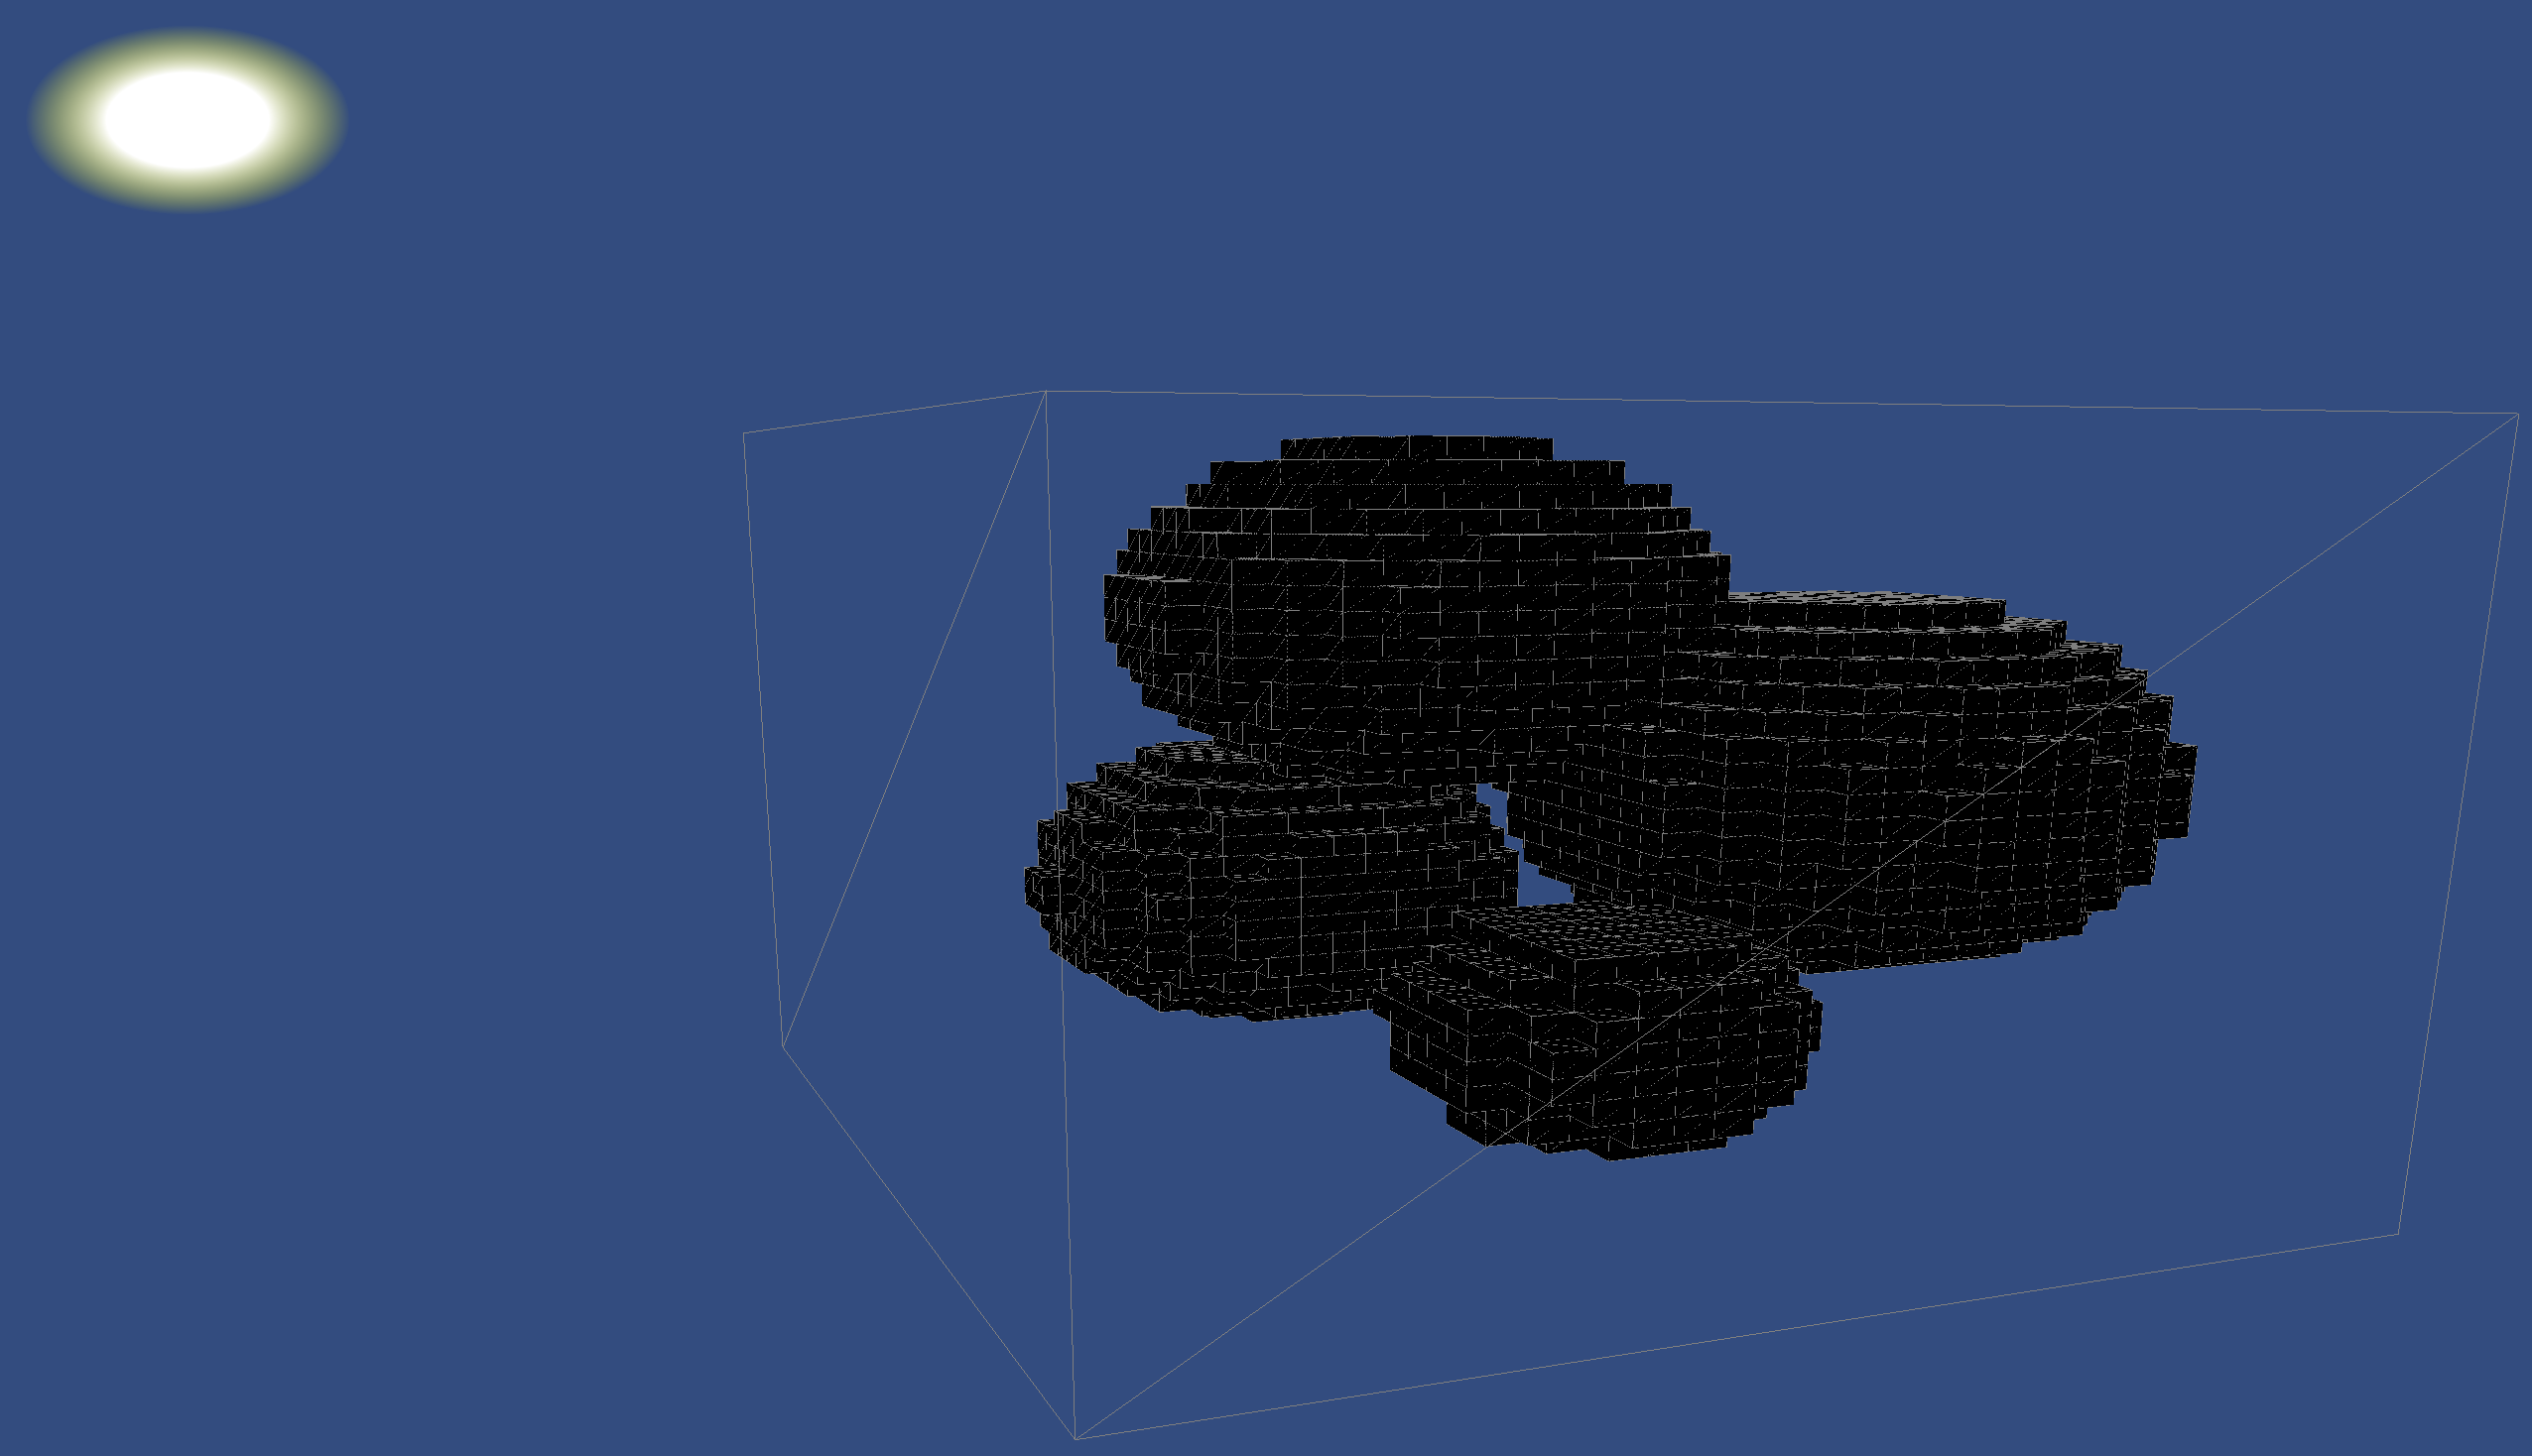
\includegraphics[width=\textwidth]{../res/voxelize1.png}
	\caption{Spherical voxelization of billboard}
	\end{subfigure}

\caption{First voxelization pass of 4 billboards}
\end{figure}

\newpage
\subsubsection{Position Map}\paragraph{}
When rendering these billboards from the light's perspective because we want to keep track of which voxels are nearest to the light source. While voxelizing, we simulatenously write the world positions of the spherical distributions into a frame buffer. 
Initially we expected the depth test to manage the occlusion of overlapping spheres. 
However, the depth test uses rasterized geometry, and our geometry being rendered is the float billboard, not the spherical representations that we want. 

To solve this, we manually update the depth buffer by calculating the fragment's spherical depth in respect to the light view's near and far plane. As of nwo this is all done in world-space, but it would be more elegant to do this calculation in clip-space.
\begin{lstlisting}[caption={first\_voxelize.glsl, 60}]
// Calculate sphere fragment's world position 
// This is the position on the sphere nearest to the light source
vec3 nearPos = fragPos + billboardNormal * sphereDistance;
// Calculate sphere fragment's depth within the light's view
float viewSize = distance(lightNearPlane, lightFarPlane);
float depth = distance(lightNearPlane, worldPos) / viewSize;
// Write position and depths to frame buffer
outColor = vec4(nearPos, 1);
gl_FragDepth = depth;
\end{lstlisting}

% Position map
\begin{figure}[t]
\centering
	% Spherical distribution mapped to a billboard
	\begin{subfigure}[t]{0.48\textwidth}
	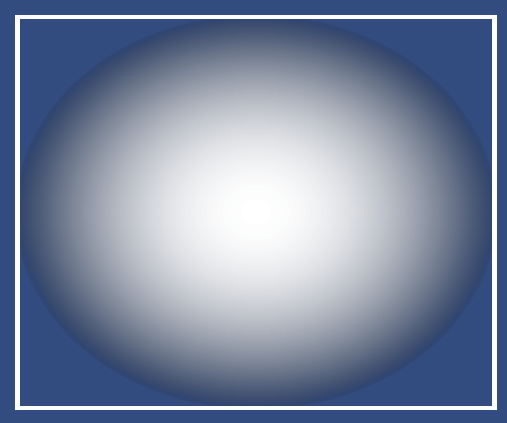
\includegraphics[width=\textwidth]{../res/spherebillboard.png}
	\caption{Spherical distribution mapped to a billboard}
	\end{subfigure}
	~
	% light-facing spherical billboard(s)
	\begin{subfigure}[t]{0.48\textwidth}
	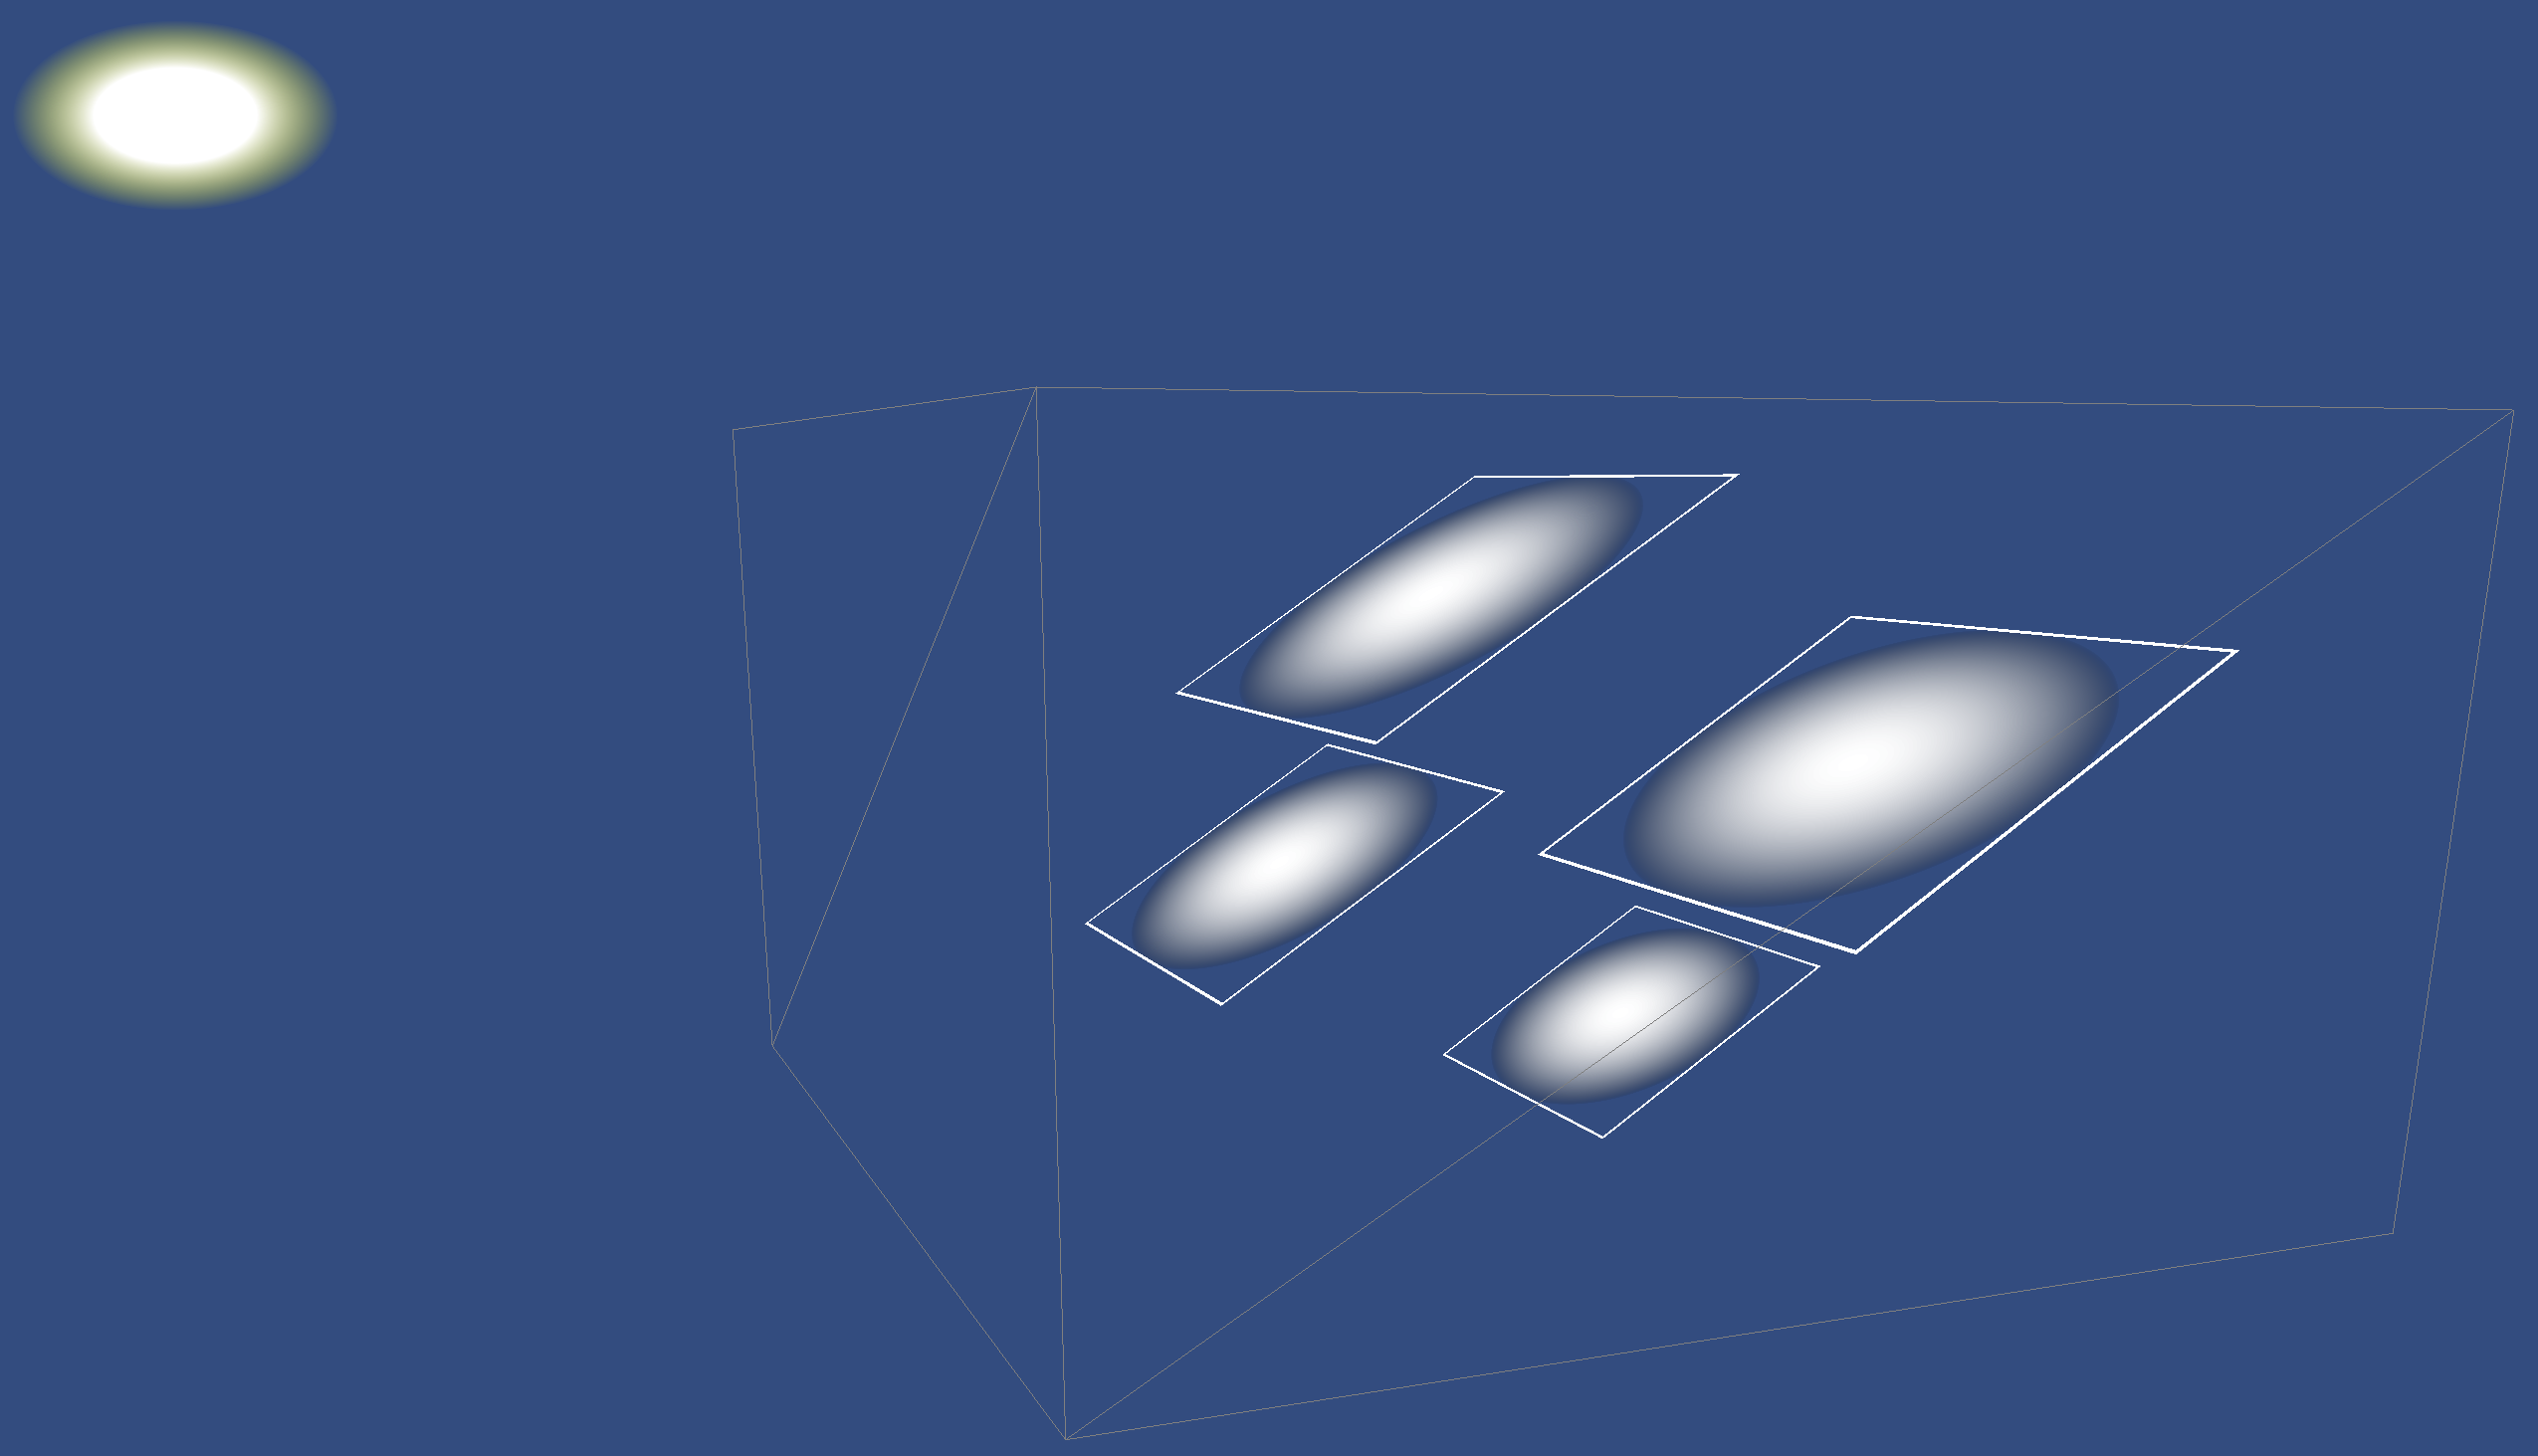
\includegraphics[width=\textwidth]{../res/lightfacing.png}
	\caption{Light-facing billboards}
	\end{subfigure}
\caption{First voxelization pass of 4 billboards}
\end{figure}

\subsubsection{Highlighting voxels}\paragraph{}
The last step for our voxelization technique is to higlight voxels nearest to the camera. Lucky for us, we have exactly what we need in the position map! 
For our second voxelization pass we render a full screen quad containing the position map. We sample each fragment of the position map to get the world positions of voxels nearest to the light source. We then update the voxel data to highlight it. 

Our result is a billowing spherical cloud-like structure with voxels nearest to the camera being highlighted. 

% img of billowing cloud

\subsubsection{Optimizations}
Because of this, our voxels only ever have three states: inactive, active, or highlighted. To optimize our approach, our voxels use R8UI as the internal format. This bits of the red channel are flipped as necessary allowing us to have minimal data representing our volume.
% light view
% rg 8?

